% Policy Wind Tunnel: project report. Build: tectonic docs/report/report.tex
\documentclass[11pt,a4paper]{article}
\usepackage[margin=2cm,top=1.8cm,bottom=2cm]{geometry}
\usepackage{fontspec}
\setmainfont{texgyrepagella}[Extension=.otf, UprightFont=*-regular, BoldFont=*-bold, ItalicFont=*-italic, BoldItalicFont=*-bolditalic]
\setsansfont{texgyreheros}[Extension=.otf, UprightFont=*-regular, BoldFont=*-bold, ItalicFont=*-italic, BoldItalicFont=*-bolditalic]
\setmonofont{lmmono10-regular}[Extension=.otf, Scale=0.95]
\usepackage{xcolor}
\definecolor{amber}{HTML}{C47600}
\definecolor{cyan}{HTML}{0E7490}
\definecolor{ink}{HTML}{1B2430}
\definecolor{muted}{HTML}{5B6673}
\definecolor{paleamber}{HTML}{FFF4E0}
\definecolor{palecyan}{HTML}{E6F6FA}
\definecolor{palegray}{HTML}{F2F4F7}
\usepackage{titlesec}
\titleformat{\section}{\sffamily\large\bfseries\color{ink}}{\thesection}{0.6em}{}
\titleformat{\subsection}{\sffamily\normalsize\bfseries\color{ink}}{\thesubsection}{0.5em}{}
\titlespacing*{\section}{0pt}{1.3ex plus .5ex}{0.6ex}
\titlespacing*{\subsection}{0pt}{1ex plus .4ex}{0.4ex}
\usepackage{booktabs,tabularx,array}
\usepackage{enumitem}
\setlist{nosep,leftmargin=1.3em,topsep=0.3ex}
\usepackage{tikz}
\usetikzlibrary{positioning,arrows.meta}
\usepackage[hidelinks]{hyperref}
\usepackage{xurl}
\urlstyle{same}
\usepackage{microtype}
\setlength{\parindent}{0pt}
\setlength{\parskip}{0.55ex}
\newcommand{\code}[1]{\texttt{#1}}
\newcommand{\hl}[1]{\textcolor{amber}{\textbf{#1}}}
\renewcommand{\arraystretch}{1.18}

\begin{document}

{\sffamily
{\small\color{cyan}\textbf{SEA × OPENAI CODEX HACKATHON VIETNAM · 31 OCTOBER 2026}}\par\vspace{0.6ex}
{\LARGE\bfseries\color{ink} Policy Wind Tunnel}\par\vspace{0.3ex}
{\large\color{muted} Test how people will read a policy before it ships}\par\vspace{0.4ex}
{\small\color{muted} Code: \url{https://github.com/beaaan/seaxopenai-hackathon}}\par}
\vspace{1ex}

\noindent\colorbox{palegray}{\parbox{\dimexpr\linewidth-2\fboxsep}{\vspace{0.6ex}
\textbf{In one paragraph.} Marketplace rules are enforced as written but acted on as understood. Policy Wind Tunnel gives the exact text of a policy to 50 simulated Vietnamese shoppers who meet it the way real buyers do (help article, checkout message, a rumour from a friend), measures what each one comes to believe, groups the misreadings and traces them to the sentence behind them. A Codex agent decides who reads next. Every proposed edit is fact-checked and re-read by the same readers, and it passes only if the improvement beats the measured test--retest noise: continuous integration for policy text. On Shopee's real COD help article, \hl{16 of 50 readers} came away believing a ``three failures in 90 days'' rule that Shopee never states. A full run costs about \textbf{\$2.56} in model calls; re-testing an edit costs about \textbf{\$0.11} and takes 17~seconds.
\vspace{0.6ex}}}

\section{The problem}

Shopee Vietnam's help article 79294 explains why cash on delivery (COD) can disappear from checkout. For the failed-delivery lock it says only that the number of unsuccessful COD deliveries in the buyer's history is
\begin{center}
\begin{minipage}{0.88\linewidth}
\itshape ``\ldots có số lượng đơn hàng COD giao không thành công \textup{\hl{vượt quá quy định hiện hành}}.''\\
\upshape\small\color{muted}(``\ldots exceeds the current rule.'') How many failures? Counted over what period? Locked for how long? The page does not say.
\end{minipage}
\end{center}
Buyers fill the gap from coupon sites and blogs: ``3 failed COD orders within 90 consecutive days locks COD'' (magiamgiashopee.vn), ``the lock lasts about 60 days'' (viettelstore.vn). None of these numbers appears in Shopee's text. The stakes are concrete:

\begin{itemize}
  \item \textbf{77.5\%} of Vietnamese e-commerce consumers choose COD~\cite{cod}, and Shopee carried \textbf{56\%} of 2025 GMV on the four largest marketplaces~\cite{metric}.
  \item \textbf{8--12\%} of online orders end in ``bom hàng'', depending on category and area~\cite{vecom}; returning a failed inter-province delivery costs the shop another \textbf{50\%} of the shipping fee~\cite{ghn}.
  \item A live support contact costs \textbf{\$8.01} on average, against about \$0.10 for self-service~\cite{gartner}.
  \item Wording measurably changes behaviour: one US Veterans Affairs letter rewrite cut related calls by \textbf{more than 80\%}~\cite{senate}.
\end{itemize}

Code is tested before release; policy text is reviewed by people who already know what it means. The existing options are slow or shallow. Paying 50 people for a one-hour interview costs about \$4{,}000 in incentives alone~\cite{ui}. A single AI review lists possible problems but cannot say \emph{how many} readers believe each one, \emph{who} they are, or \emph{whether a fix works}.

\section{What we built}

Policy Wind Tunnel is a pipeline, a CLI (\code{pwt}), an HTTP/SSE server and a web app (landing story, per-run report, live 3D replay of a run). Every stage appends to an event log; the UI, the replay and the report are all derived from that log.

\begin{figure}[h]
\centering
\resizebox{\linewidth}{!}{%
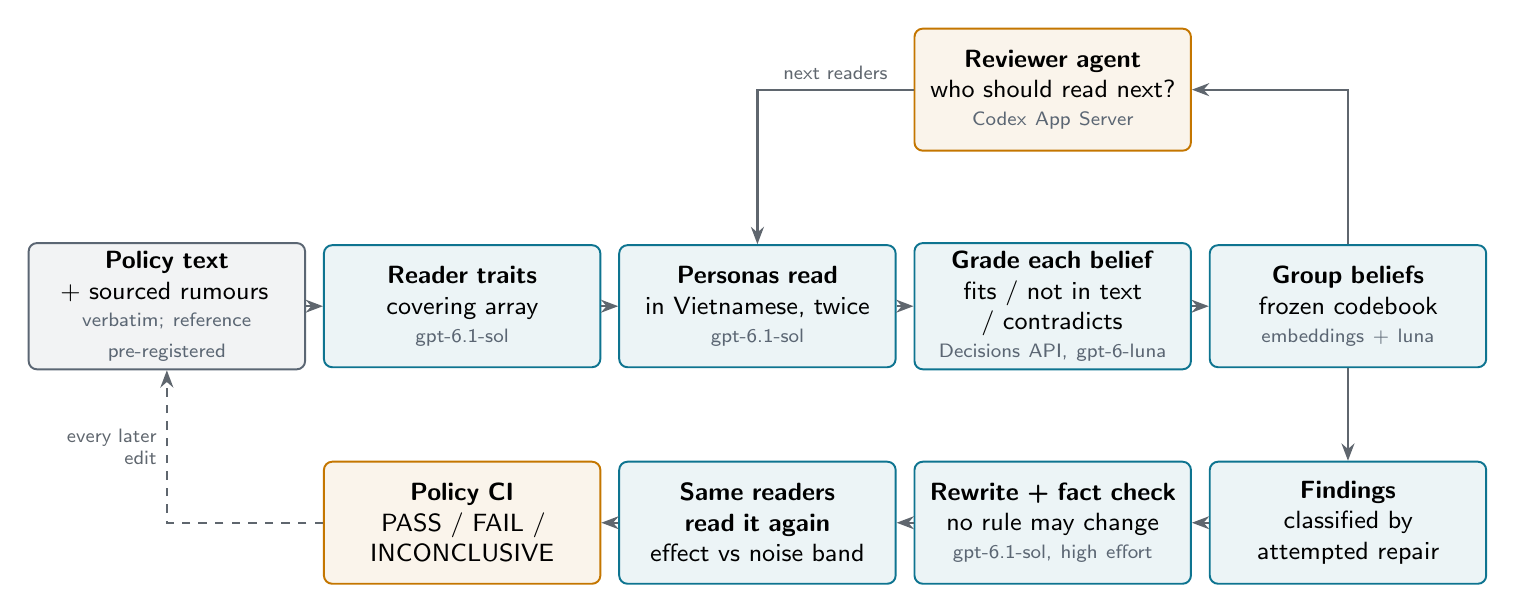
\begin{tikzpicture}[
  font=\sffamily\small,
  execute at begin node={\hyphenpenalty=10000\relax\exhyphenpenalty=10000\relax},
  box/.style={draw=#1, fill=#1!8, rounded corners=3pt, align=center, text width=3.3cm, minimum height=1.55cm, inner sep=3pt, line width=0.7pt},
  box/.default=cyan,
  arr/.style={-{Stealth[length=2.2mm]}, line width=0.8pt, color=ink!70},
  m/.style={font=\sffamily\scriptsize\color{muted}}
]
\node[box=muted] (a) at (0,0) {\textbf{Policy text}\\+ sourced rumours\\[-1pt]{\scriptsize\color{muted}verbatim; reference pre-registered}};
\node[box] (b) at (3.75,0) {\textbf{Reader traits}\\covering array\\[-1pt]{\scriptsize\color{muted}gpt-6.1-sol}};
\node[box] (c) at (7.5,0) {\textbf{Personas read}\\in Vietnamese, twice\\[-1pt]{\scriptsize\color{muted}gpt-6.1-sol}};
\node[box] (d) at (11.25,0) {\textbf{Grade each belief}\\fits / not in text / contradicts\\[-1pt]{\scriptsize\color{muted}Decisions API, gpt-6-luna}};
\node[box] (e) at (15,0) {\textbf{Group beliefs}\\frozen codebook\\[-1pt]{\scriptsize\color{muted}embeddings + luna}};
\node[box=amber] (f) at (11.25,2.75) {\textbf{Reviewer agent}\\who should read next?\\[-1pt]{\scriptsize\color{muted}Codex App Server}};
\node[box] (g) at (15,-2.75) {\textbf{Findings}\\classified by attempted repair};
\node[box] (h) at (11.25,-2.75) {\textbf{Rewrite + fact check}\\no rule may change\\[-1pt]{\scriptsize\color{muted}gpt-6.1-sol, high effort}};
\node[box] (i) at (7.5,-2.75) {\textbf{Same readers}\\\textbf{read it again}\\effect vs noise band};
\node[box=amber] (j) at (3.75,-2.75) {\textbf{Policy CI}\\PASS / FAIL / INCONCLUSIVE};
\draw[arr] (a)--(b); \draw[arr] (b)--(c); \draw[arr] (c)--(d); \draw[arr] (d)--(e);
\draw[arr] (e) |- (f); \draw[arr] (f) -| node[pos=0.25, above, m]{next readers} (c);
\draw[arr] (e)--(g); \draw[arr] (g)--(h); \draw[arr] (h)--(i); \draw[arr] (i)--(j);
\draw[arr, dashed] (j.west) -| node[pos=0.75, left, m, align=right]{every later\\edit} (a.south);
\end{tikzpicture}}
\caption{\small The pipeline. Cyan stages measure; amber stages are agents or decisions.}
\end{figure}

\vspace{-1ex}
\begin{itemize}
  \item \textbf{Readers meet the rule the way buyers do.} Besides traits extracted from the policy (payment options, shared account, delivery history), every reader has an \emph{exposure channel} (help article, checkout message only, nothing official), a \emph{prior rumour} taken from real, sourced folk versions, and an \emph{attention} level. A covering array makes every pair of trait levels appear. Readers are told to be no more careful than their persona and may be wrong.
  \item \textbf{One instrument for before and after.} Each belief is graded against reference facts that were committed before the first run. Beliefs are grouped once into a frozen codebook, and every reading of every version is coded on it (11{,}880 probability judgements in the main run), so a before/after difference is not an artefact of re-clustering.
  \item \textbf{Noise is measured, not assumed.} Every reader reads twice. An edit counts only if the change exceeds that test--retest band.
  \item \textbf{Findings are classified by trying to fix them.} A minimal rewrite is attempted and fact-checked: \emph{wording fix} if a rewrite keeps every rule and resolves it, \emph{design gap} if any fix must change a rule, \emph{unresolvable} if the text lacks the needed fact.
  \item \textbf{Policy CI.} \code{pwt test edit.json --suite <run>} re-runs the frozen suite on an edit and fails it if the fidelity check finds a new promise or a dropped fact, or if a misreading gets more common beyond noise.
\end{itemize}

\subsection{What it found (run \code{cod-main}, 50 readers, 15 minutes)}

\begin{tabularx}{\linewidth}{@{}>{\raggedright\arraybackslash}p{4.3cm}X@{}}
\toprule
\textbf{Headline} & \hl{16 of 50} readers believe a three-failure / 90-day cutoff is Shopee policy. 122 first-read beliefs $\to$ 47 groups $\to$ 7 misreadings, each traced to a sentence. \\
\textbf{The official text does not dislodge the rumour} & Of 22 readers told ``3 failures in 90 days'', 16 kept it: 3 of 5 who read the help article, 6 of 7 who saw only checkout, 7 of 10 who saw nothing official. None of the 13 readers told no rumour invented it. 11 of 15 told ``60 days'' kept expecting a 60-day lock. \\
\textbf{The obvious fix fails, and the tunnel catches it} & Adding ``this article does not state how many failures count, or over what period'' kept 10 of 10 facts with no new promise, yet belief in the cutoff moved only 0.85 $\to$ 0.82 (inside the $\pm$0.12 band) and another misreading rose from 0.17 to 0.28. Only 3 of the 10 readers ever see the help article. \emph{Conclusion: Shopee must publish the number, where buyers see it.} \\
\textbf{A bad edit is rejected} & ``Pay at a convenience store'' for cash-only buyers was rejected: the original text never promised it. \\
\textbf{A good edit passes} & Grab VN scheduled-ride terms: a rider-clause rewrite lowered the top misreading from 0.97 to 0.62 on the same 12 readers, beyond the $\pm$0.05 band, with every rule unchanged. \\
\bottomrule
\end{tabularx}

\vspace{1ex}
\begin{minipage}[t]{0.47\linewidth}
\textbf{Who misreads it} {\small\color{muted}(holders of the top misreading)}\\[0.4ex]
\small
\begin{tabularx}{\linewidth}{@{}Xr@{}}
\toprule
Heard ``3 failures in 90 days'' & \hl{16/22} \\
Heard ``locked for 60 days'' & 0/15 \\
Heard no rumour & 0/13 \\
\midrule
Saw nothing official & 7/14 \\
Saw only the checkout message & 6/18 \\
Read the help article & 3/18 \\
\midrule
Shares the account / own account & 11/27 \;·\; 5/23 \\
Skimmed / read carefully & 10/29 \;·\; 6/21 \\
\bottomrule
\end{tabularx}
\end{minipage}\hfill
\begin{minipage}[t]{0.49\linewidth}
\textbf{What one misreading can cost} {\small\color{muted}(illustrative)}\\[0.4ex]
\small
100{,}000 buyers locked out $\times$ \hl{32\%} who believe the rule (measured) $\times$ 25\% who then contact support (assumed) $\times$ \$8.01 per contact~\cite{gartner} $\approx$ \textbf{\$64{,}000}. Finding it took one run: about \textbf{\$2.56}. The landing page lets the viewer change both assumptions.
\end{minipage}

\section{Build directions}

\begin{tabularx}{\linewidth}{@{}>{\raggedright\arraybackslash}p{3.6cm}X@{}}
\toprule
\textbf{Deep Domain AI}\newline{\small\color{muted}primary} & Built on verbatim Vietnamese marketplace text and the rumours that actually circulate, with sources. Personas are Vietnamese COD shoppers who meet the rule through checkout, the help centre or a friend. The analysis separates rules the text conflates (the 24-hour daily COD cap versus the failed-delivery lock) and ends in a policy decision, not a readability score. \\
\textbf{Autonomous \& Adaptive AI} & The reviewer agent runs the sampling loop on its own: it reads where beliefs split by trait, spends the reader budget there and stops by a logged rule (new beliefs per round 9 $\to$ 5 $\to$ 5 $\to$ 2). Its 17 tool calls and every rationale are in the event log. Agent threads run isolated (empty working directory, built-in file tools off), so no persona can read the held-out answers. \\
\textbf{AI-Native Products \& Operations} & Policy CI turns a policy team's review into an automated gate: every edit is re-tested on the same readers for cents, with a PASS / FAIL / INCONCLUSIVE verdict and the evidence behind it. \\
\bottomrule
\end{tabularx}

\section{How we used LLMs}

\subsection{Inside the product}
All calls go through one gateway (cache, rate limiter, zod validation of every output, optional token log). We matched each API to the shape of the answer: labels and probabilities go to the Decisions API, generated text to Structured Outputs, agent loops judges can watch to Codex App Server.

\noindent\begin{minipage}{\linewidth}
\begin{tabularx}{\linewidth}{@{}>{\raggedright\arraybackslash}p{3.3cm}>{\raggedright\arraybackslash}p{3.9cm}Xr@{}}
\toprule
\textbf{Role} & \textbf{Model · API} & \textbf{What we ask} & \textbf{Cost\textsuperscript{*}} \\
\midrule
Readers & gpt-6.1-sol (low) · Structured Outputs & ``You are this shopper; a friend told you this; you see this screen. What do you believe now?'' & \$0.27 \\
Grader & gpt-6-luna · Decisions & Does this belief fit the policy, contradict it, or go beyond it? & \$0.02 \\
Grouping & embeddings + sol + luna & Is this belief the same idea as that one? & \$0.36 \\
Reviewer agent & gpt-6.1-sol · Codex App Server & Which trait splits beliefs? Who reads next? & \$0.10 \\
Findings, repair, fidelity & gpt-6.1-sol (high) & Name the misreading; fix it without changing a rule; did a rule change? & \$0.36 \\
Baselines + blind scoring & 3$\times$ sol, 1$\times$ gpt-6-astra & One-shot expert review, scored blind against held-out edge cases & \$0.37 \\
Persona agent & gpt-6.1-sol · Codex App Server & Live 180 simulated days under the rule; what do you do? & \$0.04 \\
\bottomrule
\end{tabularx}
{\footnotesize\color{muted}\textsuperscript{*}Measured: a fresh 20-reader run logged every call's tokens (372 calls, \$1.54 at OpenAI list prices, 10 minutes). Scaled to 50 readers, a full run is about \$2.56.}
\end{minipage}

\subsection{Building it with Codex}
\begin{itemize}
  \item \textbf{gpt-6-astra as a standing reviewer} (\code{codex exec -s read-only}): 13 logged reviews. The first, at 10:30 before any code, critiqued the plan and measurement protocol (31 items: paired noise band, frozen codebook, classification by attempted repair, blind holdout scoring). Then module-by-module code reviews, then audits of every number on the landing page against the logged runs and the cited sources.
  \item \textbf{Real catches.} App Server persona threads had inherited Codex's shell and file tools, so a persona could have read the held-out edge cases; they are now isolated. Edit re-tests were pinned to the suite's original version and input hashes. Overstated claims were corrected before the demo (for example ``more than 80\%'', not ``80\%'').
  \item \textbf{gpt-6.1-sol task agents} for self-contained slices: per-stage token metering and the cost probe, and sourced research for the stakes section (each figure with quote, date and URL; unverifiable figures were kept out).
  \item \textbf{Codex at runtime.} The reviewer and the persona agent are Codex App Server threads with our tools exposed as dynamic tools; the live replay shows their tool calls as they happened.
  \item Every Codex task is logged with its outcome in \code{docs/codex-log.md}.
\end{itemize}

\section{Limits}
Simulated readers are not a population sample: counts come from a designed mix of traits and are not national rates. The tool's job is to show which sentence to put in front of real people; the app includes a phone page for asking real buyers, coded on the same codebook. The checkout message is quoted as reported by salework.net and has not been verified in the app.

\begin{thebibliography}{9}
\setlength{\itemsep}{0pt}\small\raggedright
\newcommand{\link}[2]{\newline\href{https://#1}{\nolinkurl{#2}}}
\bibitem{cod} Ministry of Industry and Trade official, via VietnamBiz, 15/06/2025.\link{vietnambiz.vn/nghich-ly-tmdt-viet-nam-775-nguoi-tieu-dung-van-chon-thanh-toan-bang-tien-mat-khi-nhan-hang-2025615192910833.htm}{vietnambiz.vn/nghich-ly-tmdt-viet-nam-775-nguoi-tieu-dung-van-chon-thanh-toan-bang-tien-mat-khi-nhan-hang-2025615192910833.htm}
\bibitem{metric} Metric, via The Investor, 16/01/2026.\link{theinvestor.vn/online-retail-sales-in-vietnam-jump-35-to-over-16-bln-in-2025-report-d18140.html}{theinvestor.vn/online-retail-sales-in-vietnam-jump-35-to-over-16-bln-in-2025-report-d18140.html}
\bibitem{vecom} VECOM, via Người Lao Động, 19/07/2025.\link{tuoitre.vn/nld/nhuc-nhoi-nan-bom-hang-19625071822023801.htm}{tuoitre.vn/nld/nhuc-nhoi-nan-bom-hang-19625071822023801.htm}
\bibitem{ghn} Giao Hàng Nhanh, published return tariff.\link{ghn.vn/blogs/van-de-khac/don-hang-giao-khong-thanh-cong-tra-hang-thi-toi-co-mat-phi-khong}{ghn.vn/blogs/van-de-khac/don-hang-giao-khong-thanh-cong-tra-hang-thi-toi-co-mat-phi-khong}
\bibitem{gartner} Gartner, \emph{Does Your Digital Customer Service Strategy Deliver?}, 2019.\link{emt.gartnerweb.com/ngw/globalassets/en/sales-service/documents/trends/delivering-on-the-digital-promise-ebook.pdf}{emt.gartnerweb.com/ngw/globalassets/en/sales-service/documents/trends/delivering-on-the-digital-promise-ebook.pdf}
\bibitem{senate} US Senate Report 110-412, 2008.\link{www.govinfo.gov/content/pkg/CRPT-110srpt412/html/CRPT-110srpt412.htm}{govinfo.gov/content/pkg/CRPT-110srpt412/html/CRPT-110srpt412.htm}
\bibitem{ui} User Interviews, \emph{The UX Research Incentives Report}, updated 2025.\link{www.userinterviews.com/blog/research-incentives-report}{userinterviews.com/blog/research-incentives-report}
\end{thebibliography}

\end{document}
